\documentclass{ntuabeamer}

\usepackage[utf8]{inputenc}
\usepackage{amsmath}
\usepackage{appendixnumberbeamer}
\usepackage{amssymb}
\usepackage{graphicx}
\usepackage{tikz}
\usetikzlibrary{arrows.meta,calc,fit,matrix,positioning}

\title{Transformers}
\author{}
\date{}

\definecolor{courseblue}{HTML}{3F7CAC}
\definecolor{courseorange}{HTML}{D97706}
\definecolor{coursegreen}{HTML}{27864A}
\definecolor{coursegray}{HTML}{667085}
\definecolor{coursepurple}{HTML}{7656A3}
\definecolor{coursered}{HTML}{B5473C}
\definecolor{courselightblue}{HTML}{DCE9F5}
\definecolor{courselightorange}{HTML}{F9E4C8}

\newcommand{\takeaway}[1]{\par\medskip{\raggedright\color{courseblue}\bfseries #1\par}}

\tikzset{
  flow/.style={-{Latex[length=3mm]},very thick,courseblue},
  maskflow/.style={-{Latex[length=3mm]},very thick,courseorange},
  box/.style={draw,rounded corners,very thick,align=center,minimum width=1.65cm,minimum height=0.85cm},
  token/.style={draw,rounded corners,thick,align=center,minimum width=0.85cm,minimum height=0.7cm}
}

\begin{document}

\begin{frame}[plain]
  \makepresentationtitle
\end{frame}

% ---------- Motivation ----------


\section{Attention as a Soft Lookup}
\sectiondivider{Attention as a Soft Lookup}

\begin{frame}{The Problem: Distant Tokens Must Talk to Each Other}
  In ``The bridge that the inspector examined last week \textbf{is} closed'',
  the verb \emph{is} must agree with \emph{bridge}, many words earlier.
  A model needs a way to connect two tokens that are far apart.
  \begin{center}
  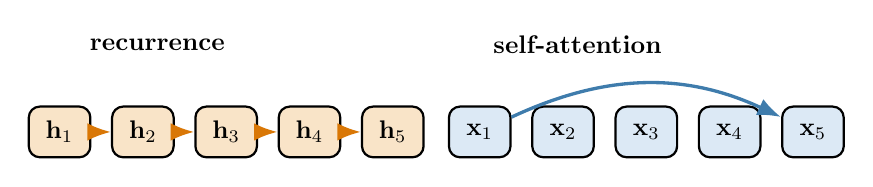
\begin{tikzpicture}[scale=0.92,transform shape]
    \node[font=\bfseries] at (2.5,2.0) {recurrence};
    \foreach \t in {1,...,5}{
      \node[token,fill=courselightorange] (r\t) at (1.15*\t,0.8) {$\mathbf h_{\t}$};
    }
    \foreach \t in {1,...,4}{
      \pgfmathtruncatemacro{\next}{\t+1}
      \draw[maskflow] (r\t) -- (r\next);
    }
    \node[font=\bfseries] at (8.3,2.0) {self-attention};
    \foreach \t in {1,...,5}{
      \node[token,fill=courselightblue] (a\t) at (5.8+1.15*\t,0.8) {$\mathbf x_{\t}$};
    }
    \draw[flow,bend left=25] (a1) to (a5);
  \end{tikzpicture}
  \end{center}
  \takeaway{So recurrence passes information along a chain of $T-1$ steps, while attention lets any token read any other directly.}
\end{frame}

\begin{frame}{The Idea: Attention Is a Soft Lookup}
  A dictionary is a \emph{hard} lookup: the query ``apple'' returns exactly one value.
  Attention is a \emph{soft} lookup: the query is compared with every key, and the answer is a
  blend of all values, weighted by how well each key matches.
  \begin{center}
  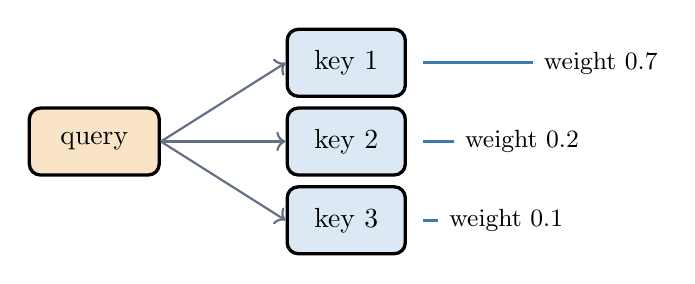
\begin{tikzpicture}[node distance=0.5cm]
    \node[box,fill=courselightorange] (q) {query};
    \foreach \i/\wt/\bw in {1/0.7/1.4,2/0.2/0.4,3/0.1/0.2}{
      \node[box,fill=courselightblue,minimum width=1.5cm] (k\i) at (3.2,1.0-1.0*\i+1) {key \i};
      \draw[courseblue,very thick] (k\i.east)++(0.2,0) -- ++(\bw,0) node[right,font=\small,black] {weight \wt};
      \draw[->,coursegray,thick] (q.east) -- (k\i.west);
    }
  \end{tikzpicture}
  \end{center}
  \takeaway{So the output is $0.7\,\mathbf v_1+0.2\,\mathbf v_2+0.1\,\mathbf v_3$: mostly the value of the best-matching key.}
\end{frame}

% ---------- Tokens, Q, K, V ----------
\begin{frame}{Tokens Become Vectors}
  A \emph{token} is one piece of the input (a word, a subword, an image patch).
  A model works with numbers, so each token becomes a vector $\mathbf x_t$ of $d_{\text{model}}$
  numbers, the model's working width. Stack the $T$ tokens as rows:
  \[
    \mathbf X=
    \begin{bmatrix}
      \mathbf x_1^{\mathsf T}\\[-1mm]
      \vdots\\[-1mm]
      \mathbf x_T^{\mathsf T}
    \end{bmatrix}
    \in\mathbb R^{T\times d_{\text{model}}}.
  \]
  \begin{center}
  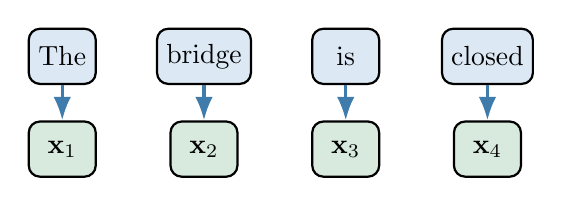
\begin{tikzpicture}[node distance=0.45cm]
    \foreach \t/\word in {1/The,2/bridge,3/is,4/closed}{
      \node[token,fill=courselightblue] (w\t) at (1.8*\t,0) {\word};
      \node[token,fill=coursegreen!18,below=of w\t] (x\t) {$\mathbf x_{\t}$};
      \draw[flow] (w\t) -- (x\t);
    }
  \end{tikzpicture}
  \end{center}
  \takeaway{So the input is a table with one row per token and one column per learned feature.}
\end{frame}

\begin{frame}{Three Roles: Query, Key, Value}
  \centering
  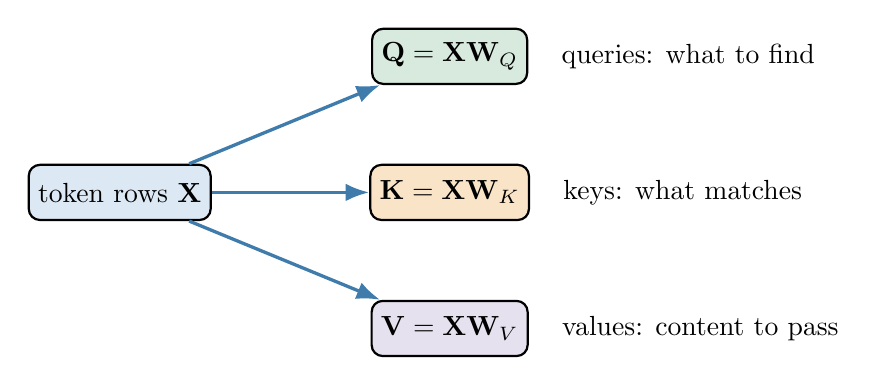
\begin{tikzpicture}[node distance=1.0cm]
    \node[token,fill=courselightblue] (x) {token rows $\mathbf X$};
    \node[token,fill=courselightorange,right=2.0cm of x] (k) {$\mathbf K=\mathbf X\mathbf W_K$};
    \node[token,fill=coursegreen!18,above=of k] (q) {$\mathbf Q=\mathbf X\mathbf W_Q$};
    \node[token,fill=coursepurple!18,below=of k] (v) {$\mathbf V=\mathbf X\mathbf W_V$};
    \draw[flow] (x)--(q); \draw[flow] (x)--(k); \draw[flow] (x)--(v);
    \node[right=0.3cm of q,align=left] {queries: what to find};
    \node[right=0.3cm of k,align=left] {keys: what matches};
    \node[right=0.3cm of v,align=left] {values: content to pass};
  \end{tikzpicture}

  \raggedright Each projection is learned. Queries and keys have width $d_k$;
  values have width $d_v$. Matching uses $Q,K$; mixing passes $V$.
\end{frame}

% ---------- Worked example in three steps ----------
\begin{frame}{Attention Step 1: Score Every Pair}
  The \emph{dot product} $\mathbf q^{\mathsf T}\mathbf k$ multiplies two vectors entry by entry and adds the results.
  It is large when the vectors point the same way and zero when they are unrelated.
  The score is $s_{ij}=\mathbf q_i^{\mathsf T}\mathbf k_j/\sqrt{d_k}$.

  \medskip
  \textbf{Example} ($d_k=2$, two tokens; the projections gave)
  \[
    \mathbf Q=\begin{bmatrix}2&0\\0&2\end{bmatrix},\quad
    \mathbf K=\begin{bmatrix}0&2\\2&0\end{bmatrix}
    \;\Rightarrow\;
    \mathbf S=\frac{\mathbf Q\mathbf K^{\mathsf T}}{\sqrt2}
    =\begin{bmatrix}0&2.83\\2.83&0\end{bmatrix}.
  \]
  Query 1 is $(2,0)$. Key 1 is $(0,2)$: dot product $0$. Key 2 is $(2,0)$: dot product $4$, score $4/\sqrt2\approx2.83$.
  \takeaway{So token 1 scores token 2 highly and itself not at all.}
\end{frame}

\begin{frame}{Attention Step 2: Softmax Turns Scores into Weights}
  \emph{Softmax} makes every score positive with $e^{s}$, then divides by the row total,
  so the weights $A_{ij}$ are positive and add up to 1.

  \medskip
  Row 1 of the example:
  \[
    e^{0}=1,\qquad e^{2.83}\approx16.9,
    \qquad
    \mathbf A_{1,:}=\Bigl(\tfrac{1}{17.9},\,\tfrac{16.9}{17.9}\Bigr)\approx(0.056,\;0.944).
  \]
  \[
    \mathbf A=\begin{bmatrix}0.056&0.944\\0.944&0.056\end{bmatrix}
  \]
  \takeaway{So token 1 puts 94\% of its attention on token 2, and token 2 does the same toward token 1.}
\end{frame}

\begin{frame}{Attention Step 3: Mix the Values}
  Each output row is the weighted average of the value rows, $\mathbf y_i=\sum_j A_{ij}\mathbf v_j$.
  With $\mathbf v_1=(1,2)$ and $\mathbf v_2=(3,0)$:
  \[
    \mathbf y_1=0.056\,(1,2)+0.944\,(3,0)\approx(2.89,\;0.11),
  \]
  \[
    \mathbf y_2=0.944\,(1,2)+0.056\,(3,0)\approx(1.11,\;1.89).
  \]
  \begin{center}
  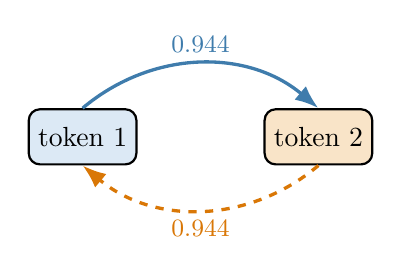
\begin{tikzpicture}[node distance=1.6cm]
    \node[token,fill=courselightblue] (t1) {token 1};
    \node[token,fill=courselightorange,right=of t1] (t2) {token 2};
    \draw[flow,bend left=40] (t1.north) to node[above,font=\small] {0.944} (t2.north);
    \draw[maskflow,bend left=40,dashed] (t2.south) to node[below,font=\small] {0.944} (t1.south);
  \end{tikzpicture}
  \end{center}
  \takeaway{So token 1's new vector is almost a copy of $\mathbf v_2$: it has retrieved what it matched.}
\end{frame}

\begin{frame}{Scaled Dot-Product Attention: The Whole Formula}
  \[
    S_{ij}=\frac{\mathbf q_i^{\mathsf T}\mathbf k_j}{\sqrt{d_k}},\qquad
    A_{ij}=\frac{e^{S_{ij}}}{\sum_r e^{S_{ir}}},\qquad
    \mathbf y_i=\sum_j A_{ij}\mathbf v_j.
  \]
  All rows at once:
  \[
    \boxed{
    \operatorname{Attn}(\mathbf Q,\mathbf K,\mathbf V)
    =\underbrace{\operatorname{softmax}_{\text{row}}
      \!\left(\frac{\mathbf Q\mathbf K^{\mathsf T}}{\sqrt{d_k}}\right)}_{\mathbf A\in\mathbb R^{T\times T}}
      \mathbf V
    }
  \]
  \begin{itemize}
    \item $\operatorname{Attn}$ names this operation; $\mathbf A$ is the table of attention weights.
    \item $\operatorname{softmax}_{\text{row}}$ applies softmax to each row separately.
    \item Row $i$ of $\mathbf A$: how much token $i$ listens to every token.
  \end{itemize}
  \takeaway{So attention = score all pairs, normalize each row, take the weighted average of the values.}
\end{frame}

\begin{frame}{Why Divide by $\sqrt{d_k}$?}
  The dot product adds $d_k$ terms, so its typical size grows with $d_k$
  (about $\sqrt{d_k}$ for unit-size entries).
  \begin{itemize}
    \item $d_k=2$: scores around $\pm1.4$, a gentle softmax.
    \item $d_k=64$: scores around $\pm8$; $e^{8}\approx3000$, so one key takes almost all the weight.
  \end{itemize}
  A near one-hot softmax has almost zero gradient, so learning stalls.
  Dividing by $\sqrt{d_k}$ keeps the typical score size near 1 for any $d_k$ (derivation in the appendix).
  \takeaway{So the scale factor stops large vectors from making the softmax saturate.}
\end{frame}

\begin{frame}{Attention Keeps One Output Per Token}
  \begin{center}
  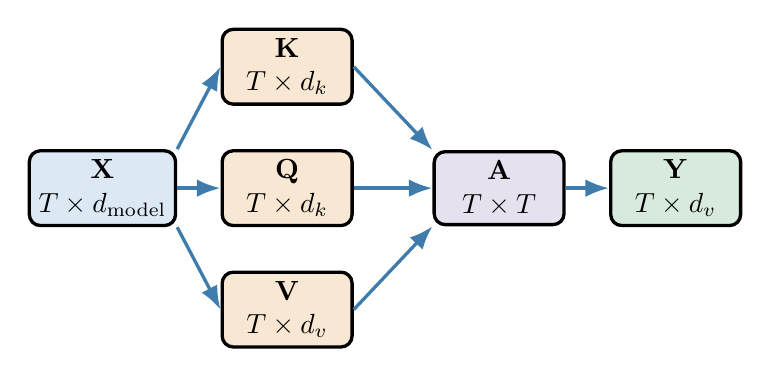
\begin{tikzpicture}[node distance=0.55cm]
    \node[box,fill=courselightblue] (x) {$\mathbf X$\\$T\times d_{\text{model}}$};
    \node[box,fill=courseorange!18,right=of x] (q) {$\mathbf Q$\\$T\times d_k$};
    \node[box,fill=courseorange!18,above=of q] (k) {$\mathbf K$\\$T\times d_k$};
    \node[box,fill=courseorange!18,below=of q] (v) {$\mathbf V$\\$T\times d_v$};
    \node[box,fill=coursepurple!18,right=1.0cm of q] (a) {$\mathbf A$\\$T\times T$};
    \node[box,fill=coursegreen!18,right=of a] (y) {$\mathbf Y$\\$T\times d_v$};
    \draw[flow] (x) -- (q);
    \draw[flow] (x.north east) -- (k.west);
    \draw[flow] (x.south east) -- (v.west);
    \draw[flow] (q) -- (a);
    \draw[flow] (k.east) -- (a.north west);
    \draw[flow] (v.east) -- (a.south west);
    \draw[flow] (a) -- (y);
  \end{tikzpicture}
  \end{center}
  \vspace{0.3cm}

  Every output row $\mathbf y_i$ belongs to one query token; the $T\times T$ matrix $\mathbf A$ holds all pairwise weights.
  \takeaway{So the sequence length stays $T$: attention updates every token using all the others.}
\end{frame}



% ---------- Multi-head ----------
\section{Heads and Word Order}
\sectiondivider{Heads and Word Order}

\begin{frame}{Why Several Heads?}
  One attention pattern per token is a limit: a word may need to look at its subject
  \emph{and} at a nearby modifier \emph{and} at a distant reference at the same time.
  \begin{center}
  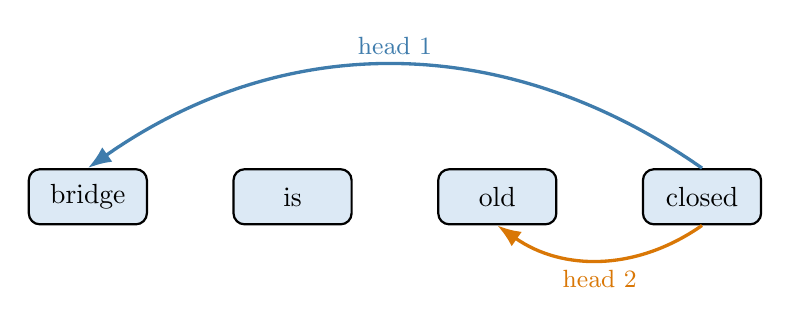
\begin{tikzpicture}[node distance=0.4cm]
    \foreach \t/\w in {1/bridge,2/is,3/old,4/closed}{
      \node[token,fill=courselightblue,minimum width=1.5cm] (t\t) at (2.6*\t,0) {\w};
    }
    \draw[flow,bend right=35] (t4.north) to node[above,font=\small] {head 1} (t1.north);
    \draw[maskflow,bend left=35] (t4.south) to node[below,font=\small] {head 2} (t3.south);
  \end{tikzpicture}
  \end{center}
  \takeaway{So we run several attention operations side by side, each free to learn a different pattern.}
\end{frame}

\begin{frame}{Multi-Head Attention}
  A \emph{head} is one independent attention operation with its own $\mathbf W_Q^{(h)},\mathbf W_K^{(h)},\mathbf W_V^{(h)}$.
  With $H$ heads, $h=1,\dots,H$:
  \[
    \mathbf Z_h=\operatorname{Attn}(\mathbf X\mathbf W_Q^{(h)},
      \mathbf X\mathbf W_K^{(h)},\mathbf X\mathbf W_V^{(h)}),
  \]
  \[
    \boxed{\operatorname{MHA}(\mathbf X)=[\mathbf Z_1\,|\,\cdots\,|\,\mathbf Z_H]\,\mathbf W_O}
  \]
  \begin{itemize}
    \item MHA = multi-head attention; $[\,\cdot\,|\,\cdot\,]$ places the head outputs side by side.
    \item $\mathbf W_O$: a learned matrix that mixes the heads and returns width $d_{\text{model}}$.
  \end{itemize}
  \takeaway{So several views are computed in parallel and merged; heads may specialize, but nothing guarantees it.}
\end{frame}

% ---------- Position ----------
\begin{frame}{Attention Alone Ignores Word Order}
  Shuffle the rows of $\mathbf X$ and attention returns the same rows, shuffled in the same way:
  $\operatorname{Attn}(\mathbf P\mathbf X)=\mathbf P\operatorname{Attn}(\mathbf X)$,
  where $\mathbf P$ is a permutation matrix (it reorders rows).
  \begin{center}
  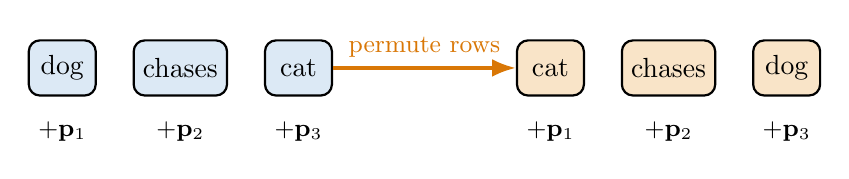
\begin{tikzpicture}[node distance=0.35cm]
    \foreach \i/\word in {1/dog,2/chases,3/cat}{
      \node[token,fill=courselightblue] (a\i) at (1.5*\i,0.7) {\word};
    }
    \foreach \i/\word in {1/cat,2/chases,3/dog}{
      \node[token,fill=courselightorange] (b\i) at (6.2+1.5*\i,0.7) {\word};
    }
    \foreach \i in {1,2,3}{
      \node[below=0.2cm of a\i,font=\small] {$+\mathbf p_{\i}$};
      \node[below=0.2cm of b\i,font=\small] {$+\mathbf p_{\i}$};
    }
    \draw[maskflow] (a3.east) -- node[above,font=\small] {permute rows} (b1.west);
  \end{tikzpicture}
  \end{center}

  Position vectors stay with slots, not words: $\widetilde{\mathbf x}_t=\mathbf x_t+\mathbf p_t$.
  \takeaway{So ``dog chases cat'' and ``cat chases dog'' look alike to attention unless we add order information.}
\end{frame}



\begin{frame}{Where Do the Position Vectors Come From?}
  \begin{itemize}
    \item \textbf{Learned}: a trained vector per position, up to the embedding table's length.
    \item \textbf{Fixed}: sinusoidal vectors computed at any position (formula in the appendix).
  \end{itemize}
  Neither choice guarantees reliable extrapolation to longer sequences.
\end{frame}



% ---------- Mask ----------
\section{The Transformer Block}
\sectiondivider{The Transformer Block}

\begin{frame}{Generating Text: A Token Must Not See the Future}
  When the model learns to predict the next word, the answer is in the data.
  If token $i$ could read tokens after it, it would just copy the answer.
  \begin{center}
  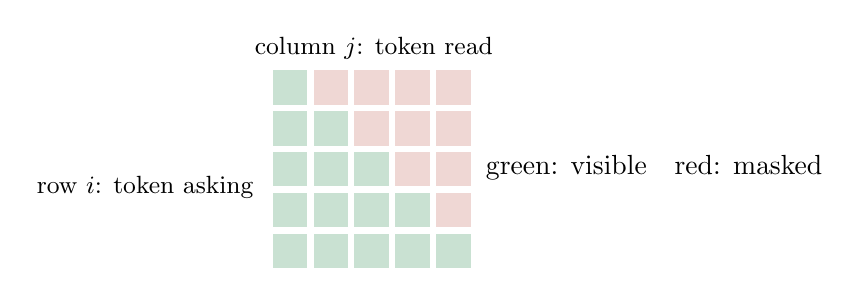
\begin{tikzpicture}[scale=0.52]
    \foreach \i in {1,...,5}{
      \foreach \j in {1,...,5}{
        \ifnum\j>\i
          \fill[coursered!22] (\j,-\i) rectangle ++(0.9,0.9);
        \else
          \fill[coursegreen!25] (\j,-\i) rectangle ++(0.9,0.9);
        \fi
        \draw[white,thick] (\j,-\i) rectangle ++(0.9,0.9);
      }
    }
    \node[right] at (6,-2.5) {green: visible\quad red: masked};
    \node[left,font=\small] at (0.8,-3) {row $i$: token asking};
    \node[above,font=\small] at (3.5,-0.1) {column $j$: token read};
  \end{tikzpicture}
  \end{center}
  \takeaway{So each token may attend only to itself and the tokens before it: the lower triangle.}
\end{frame}

\begin{frame}{The Causal Mask $\mathbf M$}
  The mask $\mathbf M$ is added to the scores: $0$ where $j\le i$, and $-\infty$ where $j>i$.
  \[
    \mathbf A=\operatorname{softmax}_{\text{row}}
      \!\left(\frac{\mathbf Q\mathbf K^{\mathsf T}}{\sqrt{d_k}}+\mathbf M\right).
  \]
  Example, token 2 with three tokens and scores $(1,\,2,\,0.5)$:
  \[
    (1,\,2,\,0.5)+(0,\,0,\,-\infty)=(1,\,2,\,-\infty)
    \;\Rightarrow\;
    \operatorname{softmax}\approx(0.27,\;0.73,\;0),
  \]
  because $e^{-\infty}=0$.
  \takeaway{So the mask gives future tokens exactly zero weight and the allowed ones still add up to 1.}
\end{frame}

% ---------- Residual / LN ----------
\begin{frame}{Deep Stacks Need a Shortcut}
  A transformer stacks many blocks. If every layer shrinks the signal a little,
  say by a factor $0.9$, then after 50 layers only $0.9^{50}\approx0.005$ of it is left,
  and gradients shrink the same way. (Illustration, not a measurement.)
  \medskip

  A \emph{residual connection} adds the block's input to its output, where $F$ is the block (attention or an MLP):
  \[
    \boxed{\mathbf Y=\mathbf X+F(\mathbf X)}
  \]
  \takeaway{So the input always has a direct path forward, even if the learned update $F$ is small.}
\end{frame}

\begin{frame}{Residual Connection: Picture}
  \begin{center}
  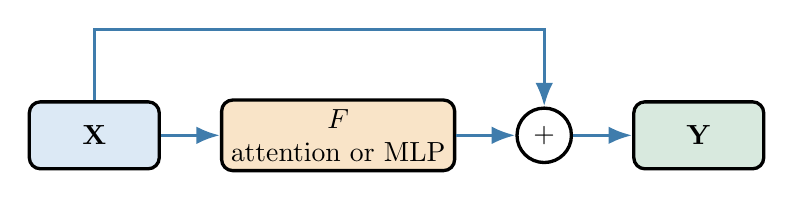
\begin{tikzpicture}[node distance=0.75cm]
    \node[box,fill=courselightblue] (x) {$\mathbf X$};
    \node[box,fill=courselightorange,right=of x] (f) {$F$\\attention or MLP};
    \node[draw,circle,very thick,right=of f] (plus) {$+$};
    \node[box,fill=coursegreen!18,right=of plus] (y) {$\mathbf Y$};
    \draw[flow] (x) -- (f);
    \draw[flow] (f) -- (plus);
    \draw[flow] (plus) -- (y);
    \draw[flow] (x.north) -- ++(0,0.9) -| (plus.north);
  \end{tikzpicture}
  \end{center}

  \begin{itemize}
    \item Top path: the input skips the block unchanged.
    \item Bottom path: the block computes a correction $F(\mathbf X)$.
    \item In backpropagation the skip path hands gradients straight back to earlier layers.
  \end{itemize}
  \takeaway{So each block learns a correction to its input rather than a whole new representation; residuals help training but do not by themselves guarantee stability.}
\end{frame}

\begin{frame}{Layer Normalization: Keeping Features on One Scale}
  Feature values can drift to very different sizes from layer to layer.
  \emph{Layer normalization} (LN) rescales each token's own feature vector:
  subtract its mean, divide by its standard deviation.

  \medskip
  Example, token $(2,4,6,8)$: mean $5$, standard deviation $\sqrt5\approx2.24$,
  \[
    (2,4,6,8)\;\mapsto\;(-1.34,\,-0.45,\,0.45,\,1.34).
  \]
  \takeaway{So every token leaves LN with mean 0 and spread 1, whatever its original scale.}
\end{frame}

\begin{frame}{Layer Normalization: Learned Scale and Where It Sits}
  After normalizing, LN applies a learned per-feature scale $\boldsymbol\gamma$ and shift $\boldsymbol\beta$,
  so the model can undo the normalization where that helps; a tiny constant $\varepsilon$ avoids division by zero
  (full formula in the appendix).

  \medskip
  In a ``pre-norm'' block, LN is applied before the sublayer $F$ and the residual path is left untouched:
  \[
    \boxed{\mathbf Y=\mathbf X+F(\operatorname{LN}(\mathbf X))}.
  \]
  Statistics are computed per token, never pooled across tokens or across a batch.
  \takeaway{So LN stabilizes each sublayer's input while the residual path stays clean.}
\end{frame}

% ---------- Blocks ----------
\begin{frame}{The Position-Wise MLP}
  Attention mixes information \emph{between} tokens. Something must also process
  each token's features on their own: the \emph{MLP block}.
  \begin{itemize}
    \item Two dense layers with a nonlinearity in between: widen, apply the nonlinearity, shrink back to $d_{\text{model}}$.
    \item ``Position-wise'': the same weights are applied to every token row independently.
  \end{itemize}
  \begin{center}
    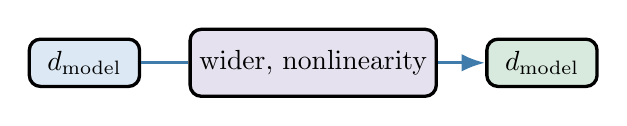
\begin{tikzpicture}[node distance=0.6cm]
      \node[box,fill=courselightblue,minimum width=1.4cm,minimum height=0.6cm] (a) {$d_{\text{model}}$};
      \node[box,fill=coursepurple!18,minimum width=2.6cm,right=of a] (b) {wider, nonlinearity};
      \node[box,fill=coursegreen!18,minimum width=1.4cm,minimum height=0.6cm,right=of b] (c) {$d_{\text{model}}$};
      \draw[flow] (a)--(b)--(c);
    \end{tikzpicture}
  \end{center}
  \takeaway{So attention moves information across tokens, and the MLP then transforms each token's features.}
\end{frame}

\begin{frame}{An Encoder Block Mixes Tokens, Then Features}
  \begin{center}
  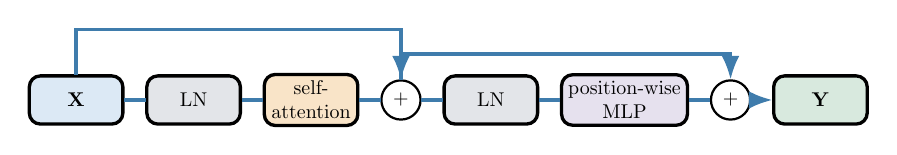
\begin{tikzpicture}[node distance=0.38cm,scale=0.72,transform shape]
    \node[box,fill=courselightblue] (x) {$\mathbf X$};
    \node[box,fill=coursegray!18,right=of x] (ln1) {LN};
    \node[box,fill=courselightorange,right=of ln1] (mha) {self-\\attention};
    \node[draw,circle,thick,right=of mha] (p1) {$+$};
    \node[box,fill=coursegray!18,right=of p1] (ln2) {LN};
    \node[box,fill=coursepurple!18,right=of ln2] (ffn) {position-wise\\MLP};
    \node[draw,circle,thick,right=of ffn] (p2) {$+$};
    \node[box,fill=coursegreen!18,right=of p2] (y) {$\mathbf Y$};
    \draw[flow] (x)--(ln1)--(mha)--(p1)--(ln2)--(ffn)--(p2)--(y);
    \draw[flow] (x.north) -- ++(0,0.8) -| (p1.north);
    \draw[flow] (p1.north) -- ++(0,0.45) -| (p2.north);
  \end{tikzpicture}
  \end{center}

  \vspace{0.3cm}
  Read left to right: normalize, attend, add the skip; normalize, MLP, add the skip.
  \takeaway{So a block is attention plus MLP, each wrapped with LN and a residual; deep models repeat this block.}
\end{frame}

\begin{frame}{A Decoder Block Uses Masked Self-Attention}
  \begin{center}
  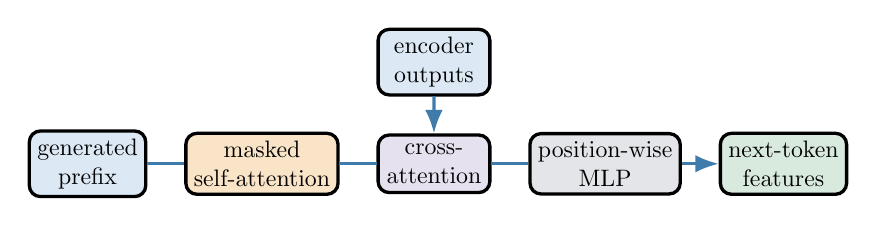
\begin{tikzpicture}[node distance=0.55cm,scale=0.86,transform shape]
    \node[box,fill=courselightblue] (x) {generated\\prefix};
    \node[box,fill=courselightorange,right=of x] (self) {masked\\self-attention};
    \node[box,fill=coursepurple!18,right=of self] (cross) {cross-\\attention};
    \node[box,fill=coursegray!18,right=of cross] (ffn) {position-wise\\MLP};
    \node[box,fill=coursegreen!18,right=of ffn] (y) {next-token\\features};
    \node[box,fill=courselightblue,above=of cross] (enc) {encoder\\outputs};
    \draw[flow] (x)--(self)--(cross)--(ffn)--(y);
    \draw[flow] (enc)--(cross);
  \end{tikzpicture}
  \end{center}

  \vspace{0.3cm}
  The decoder is the generating side. Cross-attention (next frame) exists only in encoder--decoder models;
  decoder-only language models drop it and the encoder.
  \takeaway{So a decoder block is an encoder block with a causal mask, plus optional cross-attention.}
\end{frame}

\begin{frame}{Cross-Attention Connects Two Streams}
  Same attention operation, but the queries come from one stream (the target)
  and the keys and values from another (the source):
  \[
    \mathbf Q=\mathbf X_{\text{target}}\mathbf W_Q,
    \qquad
    \mathbf K=\mathbf X_{\text{source}}\mathbf W_K,
    \qquad
    \mathbf V=\mathbf X_{\text{source}}\mathbf W_V.
  \]
  \begin{center}
  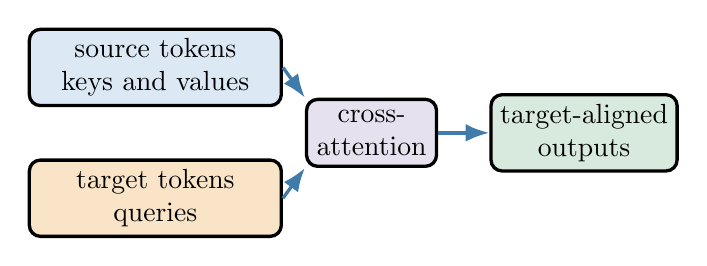
\begin{tikzpicture}[node distance=0.65cm]
    \node[box,fill=courselightblue,minimum width=3.2cm] (source) {source tokens\\keys and values};
    \node[box,fill=courselightorange,minimum width=3.2cm,below=of source] (target) {target tokens\\queries};
    \node[box,fill=coursepurple!18,right=1.9cm of $(source)!0.5!(target)$] (attn) {cross-\\attention};
    \node[box,fill=coursegreen!18,right=of attn] (out) {target-aligned\\outputs};
    \draw[flow] (source.east) -- (attn.north west);
    \draw[flow] (target.east) -- (attn.south west);
    \draw[flow] (attn) -- (out);
  \end{tikzpicture}
  \end{center}
  \takeaway{So in translation each target word retrieves the source words it needs; the same idea connects text with images.}
\end{frame}



% ---------- Language modelling ----------
\section{Language Models, Cost and Limits}
\sectiondivider{Language Models, Cost and Limits}

\begin{frame}{Language Models Predict the Next Token}
  Given the tokens so far, the model outputs a probability for every possible next token.
  (Illustrative numbers.)
  \begin{center}
  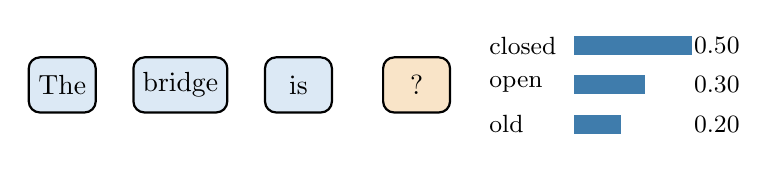
\begin{tikzpicture}[node distance=0.4cm]
    \node[token,fill=courselightblue] (a) at (0,0) {The};
    \node[token,fill=courselightblue] (b) at (1.5,0) {bridge};
    \node[token,fill=courselightblue] (c) at (3.0,0) {is};
    \node[token,fill=courselightorange] (d) at (4.5,0) {?};
    \foreach \w/\p/\y in {closed/0.50/0.5,open/0.30/0,old/0.20/-0.5}{
      \node[right,font=\small] at (5.3,\y) {\w};
      \fill[courseblue] (6.5,\y-0.12) rectangle ++(3*\p,0.24);
      \node[right,font=\small] at (7.9,\y) {\p};
    }
  \end{tikzpicture}
  \end{center}
  \takeaway{So a language model is a machine that turns a prefix into a distribution over the next token.}
\end{frame}

\begin{frame}{Autoregressive Factorization and the Training Loss}
  Chain the next-token predictions, with $x_{<t}=(x_1,\dots,x_{t-1})$ the tokens before $t$:
  \[
    \boxed{p(x_{1:T})=\prod_{t=1}^{T}p(x_t\mid x_{<t})}
  \]
  Training minimizes the negative log-probability of the true tokens:
  $L(\boldsymbol\theta)=-\sum_{t}\log p_{\boldsymbol\theta}(x_t\mid x_{<t})$.

  \medskip
  Example: true tokens given probability $0.5,\,0.2,\,0.4$:
  product $0.04$; loss $0.69+1.61+0.92=3.22$.
  \takeaway{So the loss is small when the model gives high probability to every true next token; the factorization is exact, the learned conditionals are approximate.}
\end{frame}

\begin{frame}{Training Is Parallel; Generation Is Sequential}
  \begin{center}
  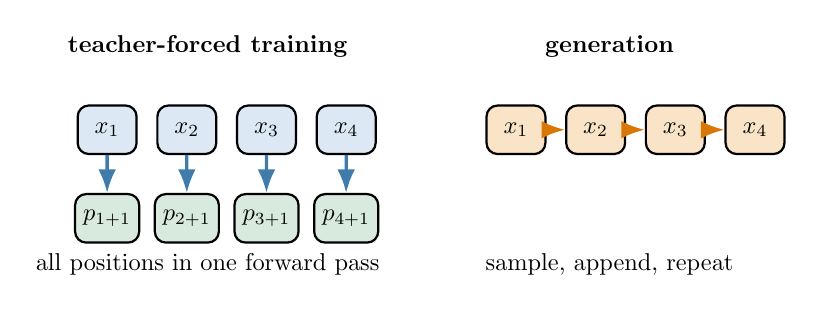
\begin{tikzpicture}[scale=0.88,transform shape]
    \node[font=\bfseries] at (2.6,2.0) {teacher-forced training};
    \foreach \t in {1,...,4}{
      \node[token,fill=courselightblue] (tr\t) at (1.15*\t,0.8) {$x_{\t}$};
      \node[token,fill=coursegreen!18,below=0.55cm of tr\t] (pr\t) {$p_{\t+1}$};
      \draw[flow] (tr\t)--(pr\t);
    }
    \node at (2.6,-1.15) {all positions in one forward pass};
    \node[font=\bfseries] at (8.4,2.0) {generation};
    \foreach \t in {1,...,4}{
      \node[token,fill=courselightorange] (g\t) at (5.9+1.15*\t,0.8) {$x_{\t}$};
    }
    \foreach \t in {1,...,3}{
      \pgfmathtruncatemacro{\next}{\t+1}
      \draw[maskflow] (g\t)--(g\next);
    }
    \node at (8.4,-1.15) {sample, append, repeat};
  \end{tikzpicture}
  \end{center}

  Teacher forcing: the true previous tokens are fed in, so every position predicts its next token at once
  ($p_{t+1}$ = predicted distribution for token $t+1$). At generation time the next token is unknown.
  \takeaway{So training can use all positions together, but generation must produce one token at a time.}
\end{frame}

% ---------- Cost, scope, limits ----------
\begin{frame}{Dense Attention Has Quadratic Cost}
  The score matrix $\mathbf Q\mathbf K^{\mathsf T}$ has one entry for every pair of tokens.
  \begin{center}
  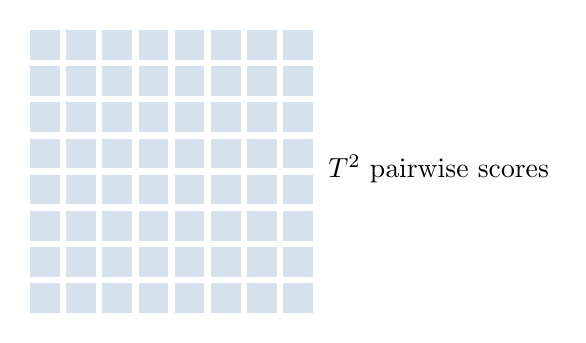
\begin{tikzpicture}[scale=0.46]
    \foreach \i in {1,...,8}{
      \foreach \j in {1,...,8}{
        \fill[courseblue!22] (\i,-\j) rectangle ++(0.88,0.88);
        \draw[white,thick] (\i,-\j) rectangle ++(0.88,0.88);
      }
    }
    \node[right] at (9,-4) {$T^2$ pairwise scores};
  \end{tikzpicture}
  \end{center}
  \begin{itemize}
    \item $T=1000$: $10^6$ scores. $T=2000$: $4\times10^6$.
    \item $T=100\,000$: $10^{10}$ scores, about 40~GB in 32-bit floats for a single head of a single layer (if stored).
  \end{itemize}
  \takeaway{So doubling the length quadruples the cost, which is why long contexts need sparse or local attention variants.}
\end{frame}

\begin{frame}{A Token Can Represent More Than a Word}
  \begin{center}
  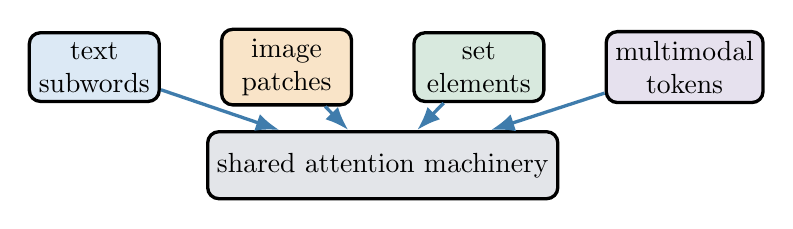
\begin{tikzpicture}[node distance=0.75cm]
    \node[box,fill=courselightblue] (text) {text\\subwords};
    \node[box,fill=courselightorange,right=of text] (image) {image\\patches};
    \node[box,fill=coursegreen!18,right=of image] (set) {set\\elements};
    \node[box,fill=coursepurple!18,right=of set] (multi) {multimodal\\tokens};
    \node[box,fill=coursegray!18,below=0.8cm of $(image)!0.5!(set)$] (block) {shared attention machinery};
    \draw[flow] (text)--(block);
    \draw[flow] (image)--(block);
    \draw[flow] (set)--(block);
    \draw[flow] (multi)--(block);
  \end{tikzpicture}
  \end{center}

  \vspace{0.3cm}
  The tokenizer decides what one row of $\mathbf X$ means, and the position scheme must match the domain
  (a sequence, a 2-D grid of patches, or an unordered set).
  \takeaway{So attention is a general interaction rule; the choice of tokens and positions supplies the structure of the problem.}
\end{frame}

\begin{frame}{Attention Weights Are Not Automatically Explanations}
  It is tempting to read the heat map $A_{ij}$ as ``why the model decided''.
  \begin{itemize}
    \item $A_{ij}$ is a weight inside one attention operation.
    \item Values, output projections, residual paths, and later layers also shape the prediction.
    \item Different heads may distribute weight differently.
  \end{itemize}
  \begin{center}
  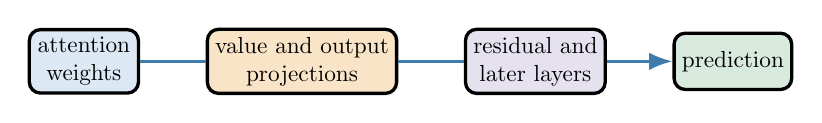
\begin{tikzpicture}[scale=0.84,transform shape]
    \node[box,fill=courselightblue] (weights) {attention\\weights};
    \node[box,fill=courselightorange,right=of weights] (values) {value and output\\projections};
    \node[box,fill=coursepurple!18,right=of values] (layers) {residual and\\later layers};
    \node[box,fill=coursegreen!18,right=of layers] (prediction) {prediction};
    \draw[flow] (weights)--(values)--(layers)--(prediction);
  \end{tikzpicture}
  \end{center}
  \takeaway{So a plausible-looking attention map is a clue, not evidence of causal importance.}
\end{frame}

\begin{frame}{Transformers Still Have Important Failure Modes}
  \begin{itemize}
    \item Context is finite; relevant information may be absent or poorly used.
    \item Dense attention becomes expensive for long sequences.
    \item Position schemes may extrapolate poorly beyond training lengths.
    \item Learned correlations can reproduce bias and generate unsupported claims.
  \end{itemize}
  \begin{center}
  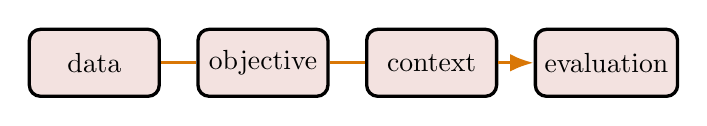
\begin{tikzpicture}[node distance=0.45cm]
    \node[box,fill=coursered!16] (data) {data};
    \node[box,fill=coursered!16,right=of data] (objective) {objective};
    \node[box,fill=coursered!16,right=of objective] (context) {context};
    \node[box,fill=coursered!16,right=of context] (evaluation) {evaluation};
    \draw[maskflow] (data)--(objective)--(context)--(evaluation);
  \end{tikzpicture}
  \end{center}
  \takeaway{So large capacity does not remove the need for validation: check the data, the objective, the context and the evaluation.}
\end{frame}



\appendix
\sectiondivider{Appendix: optional depth}

\begin{frame}{Appendix: Why Divide by $\sqrt{d_k}$}
  Assume independent, zero-mean query and key coordinates with unit variance.
  \[
    s=\mathbf q^{\mathsf T}\mathbf k=\sum_{r=1}^{d_k}q_rk_r,
    \qquad
    \mathbb E[s]=0,
    \qquad
    \operatorname{Var}(s)=d_k.
  \]
  Therefore,
  \[
    \operatorname{Var}\!\left(\frac{s}{\sqrt{d_k}}\right)=1.
  \]
  \begin{itemize}
    \item Unscaled logits grow in typical magnitude with dimension.
    \item Very large logits can saturate the softmax, leaving tiny gradients.
    \item This is an initialization-scale heuristic, not a theorem about trained activations.
  \end{itemize}
\end{frame}

\begin{frame}{Appendix: Layer Normalization Formula}
  For one token vector $\mathbf x\in\mathbb R^d$ with entries $x_j$,
  \[
    \mu=\frac1d\sum_{j=1}^{d}x_j,
    \qquad
    \sigma^2=\frac1d\sum_{j=1}^{d}(x_j-\mu)^2,
  \]
  \[
    \operatorname{LN}(\mathbf x)
    =\boldsymbol\gamma\odot
      \frac{\mathbf x-\mu\mathbf 1}{\sqrt{\sigma^2+\varepsilon}}
      +\boldsymbol\beta.
  \]
  \begin{itemize}
    \item $\mu,\sigma^2$: mean and variance of the $d$ features of this token.
    \item $\mathbf 1$ is the all-ones vector; $\odot$ multiplies entry by entry.
    \item $\boldsymbol\gamma,\boldsymbol\beta\in\mathbb R^d$ are learned scale and shift; $\varepsilon$ is a tiny constant (for example $10^{-5}$).
  \end{itemize}
\end{frame}

\begin{frame}{Appendix: Sinusoidal Position Vectors}
  A fixed choice for $\mathbf p_t$ (entries $2i$ and $2i{+}1$ of the vector for position $t$):
  \[
    p_{t,2i}=\sin\!\left(t/10000^{2i/d_{\text{model}}}\right),
    \qquad
    p_{t,2i+1}=\cos\!\left(t/10000^{2i/d_{\text{model}}}\right).
  \]
  Example with $d_{\text{model}}=4$: $\mathbf p_t=(\sin t,\cos t,\sin 0.01t,\cos 0.01t)$.
  \[
    \mathbf p_1\approx(0.84,\,0.54,\,0.01,\,1.00),\qquad
    \mathbf p_2\approx(0.91,\,-0.42,\,0.02,\,1.00).
  \]
  \begin{itemize}
    \item Each pair of entries is a sine--cosine wave; the wavelength grows with $i$.
    \item Every position gets a distinct pattern, and nothing is learned.
    \item It is defined for any $t$, but that is not a guarantee of good extrapolation.
  \end{itemize}
\end{frame}

\end{document}
